%{{{ preamble
\documentclass[a4paper,9pt]{article}
\usepackage{anysize}
\marginsize{2cm}{2cm}{1cm}{1cm}
%\textwidth 6.0in \textheight = 664pt
\usepackage{xltxtra}
\usepackage{xunicode}
\usepackage{graphicx}
\usepackage{color}
\usepackage{xgreek}
\usepackage{fancyvrb}
\usepackage{minted}
\usepackage{listings}
\usepackage{enumitem} 
\usepackage{framed} 
\usepackage{relsize}
\usepackage{float} 
\usepackage{pstricks}
\usepackage{pst-node}
\usepackage{pst-blur}
\setmainfont[Mapping=tex-text]{FreeSerif}
%}}}
\begin{document}

\def\thesection {Μέρος \alph{section}}
\def\thesubsection {\roman{subsection}.}

\begin{titlepage}
\begin{center}
\begin{figure}[h] 
     
\includegraphics[width=0.2\textwidth]{title/ntua_logo}
\end{figure}
\vspace{1cm}
\begin{LARGE}\textbf{ΕΘΝΙΚΟ ΜΕΤΣΟΒΙΟ ΠΟΛΥΤΕΧΝΕΙΟ\\[1.5cm]}\end{LARGE}
\begin{Large}
ΣΧΟΛΗ ΗΜ\&ΜΥ\\
Διαδίκτυο \& Εφαρμογές\\[2cm]
1\textsuperscript{η} Άσκηση\\
Ακ. έτος 2011-2012\\
\end{Large}
\vfill
\begin{flushright}
\begin{tabular}{l r}
{Γρηγόρης \textsc{Λύρας}}&
{Α.Μ.: 03109687}\\
\end{tabular}
\end{flushright}

\large\today\\
\end{center}
\end{titlepage}





\section{Οθόνες}
\begin{figure}[H]
    \centering
    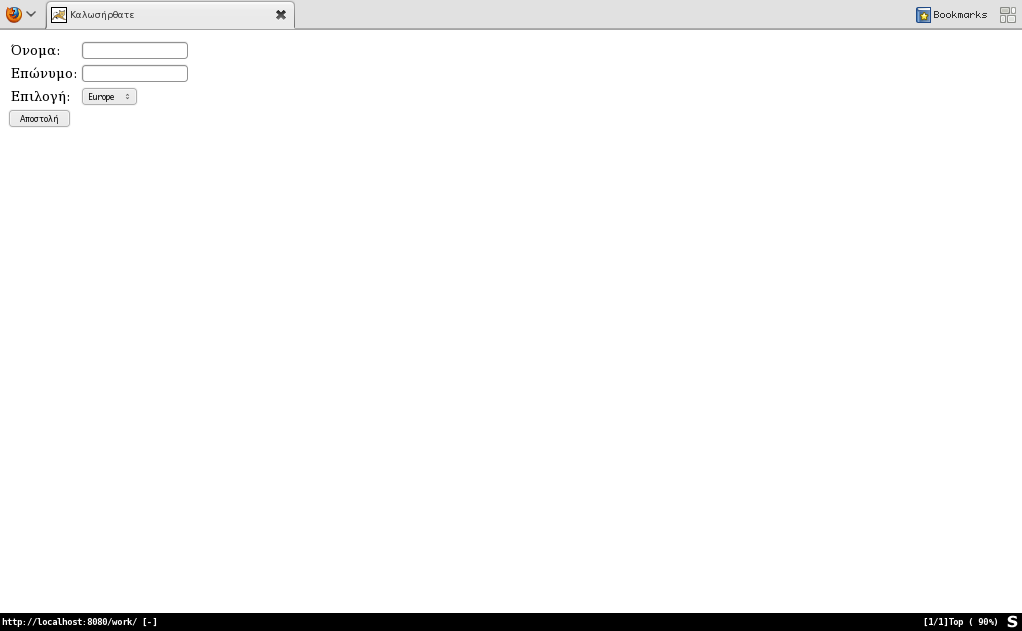
\includegraphics[width=0.9\textwidth]{files/1.png}
    \caption{Αρχική σελίδα}
\end{figure}

Στην αρχική σελίδα εισάγει ο χρήστης τα στοιχεία του και επιλέγει αν επιθυμεί
να ταξιδέψει στην Ευρώπη ή στην Ασία.
\begin{figure}[H]
    \centering
    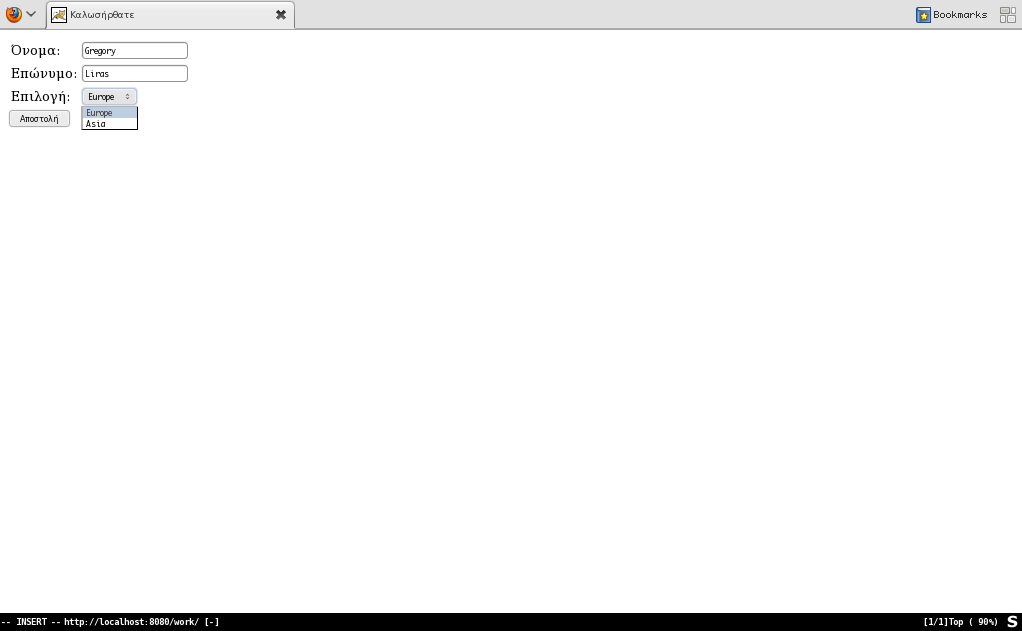
\includegraphics[width=0.9\textwidth]{files/2.png}
    \caption{Αρχική σελίδα (γεμάτη)}
\end{figure}

Αφού συμπληρώσει τα στοιχεία του πατάει το κουμπί Submit και αυτά αποστέλονται
με POST στην επόμενη σελίδα.
\begin{figure}[H]
    \centering
    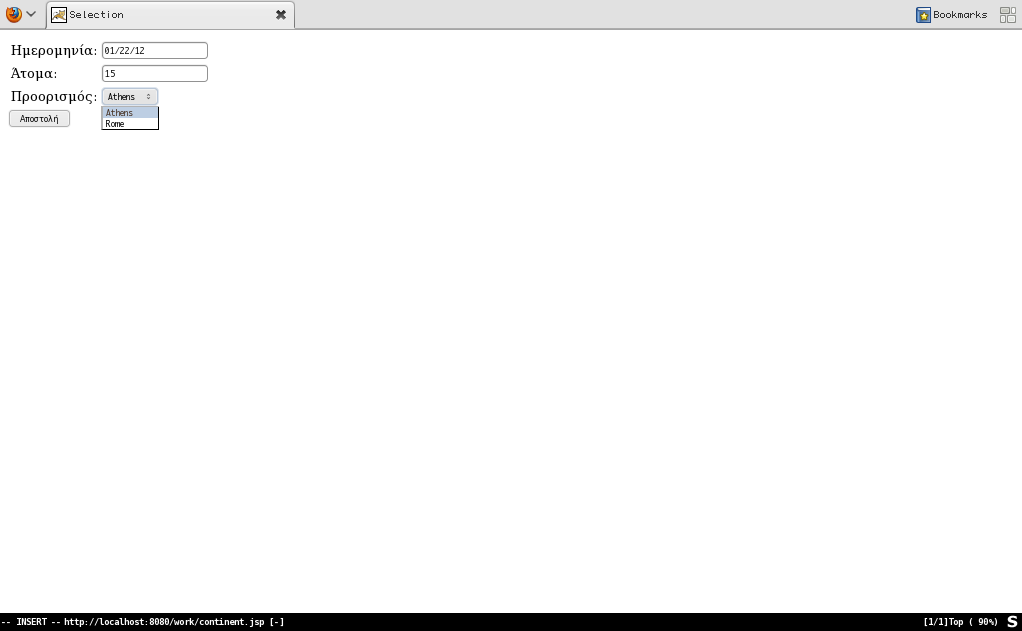
\includegraphics[width=0.9\textwidth]{files/3.png}
    \caption{Δεύτερη σελίδα (γεμάτη)}
\end{figure}
Στη δεύτερη σελίδα ο χρήστης συμπληρώνει την ημερομηνία που επιθυμεί να
ταξιδέψει καθώς και το πλήθος των ατόμων.
\begin{figure}[H]
    \centering
    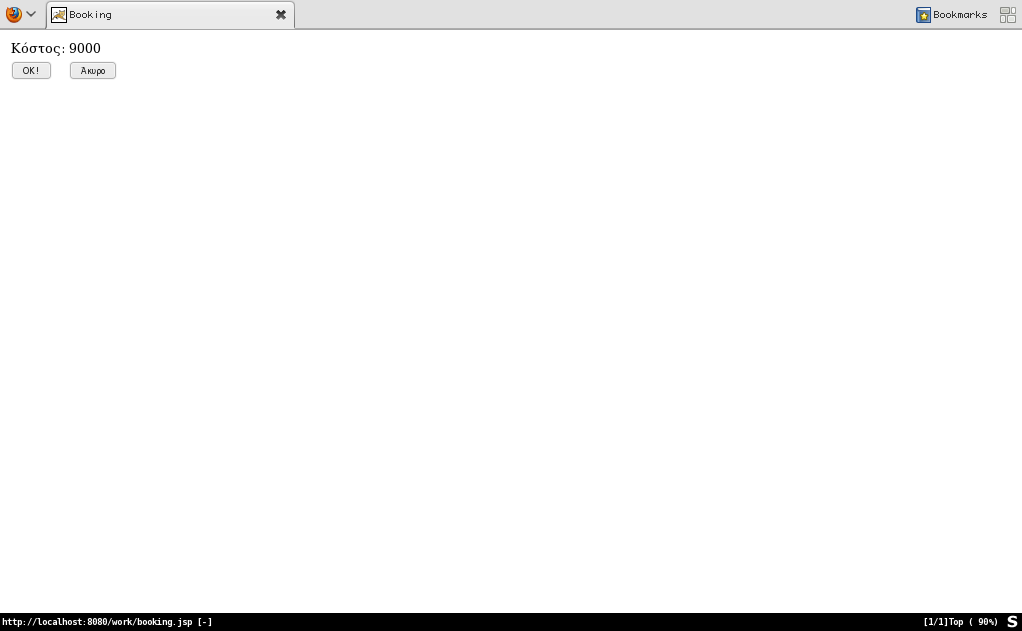
\includegraphics[width=0.9\textwidth]{files/4.png}
    \caption{Υπολογισμός κόστους και επιλογή χρήστη  (άκυρο)}
\end{figure}
Σύμφωνα με τον προορισμό και το πλήθος των ατόμων υπολογίζουμε το κόστος του
ταξιδιού και δίνουμε στο χρήστη την επιλογή να αποδεχτεί την παραγγελία είτε
να την ακυρώσει.
\begin{figure}[H]
    \centering
    \includegraphics[width=0.9\textwidth]{files/5.png}
    \caption{Επιστροφή στην προηγούμενη σελίδα}
\end{figure}
Εάν την ακυρώσει βρίσκεται στην αμέσως προηγούμενη σελίδα όπου και του δίνεται
η δυνατότητα να επιλέξει πάλι προορισμό, πλήθος ατόμων και ημερομηνία αν
επιθυμεί.
\begin{figure}[H]
    \centering
    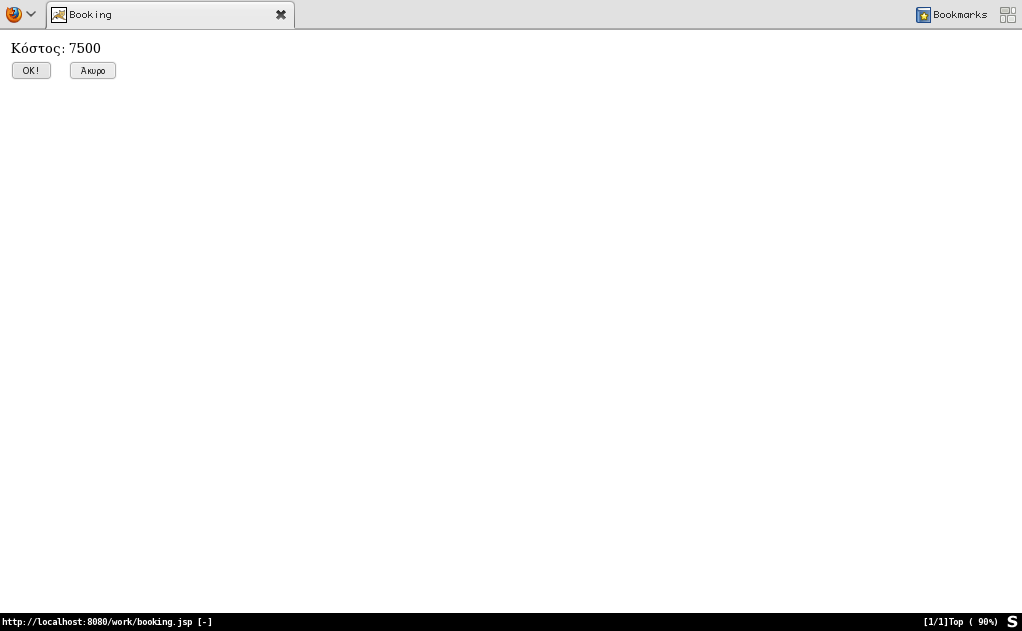
\includegraphics[width=0.9\textwidth]{files/6.png}
    \caption{Νέο κόστος}
\end{figure}
Επανυπολογίζουμε το κόστος και αφού ο χρήστης επιβεβαιώσει ολοκληρώνεται η
παραγγελία.
\begin{figure}[H]
    \centering
    \includegraphics[width=0.9\textwidth]{files/7.png}
    \caption{Τελική σελίδα}
\end{figure}
Στην τελική σελίδα, παρουσιάζονται στον χρήστη όλες οι προηγούμενες επιλογές
του σαν τελικό δελτίο παραγγελίας. Ακόμη δίνεται στο χρήστη η επιλογή να
ξαναξεκινήσει τη διαδικασία για νέα παραγγελία αν το επιθυμεί.  Ακόμη
σβήνονται όλα τα cookies και οι φόρμες είναι και πάλι καθαρές.
\begin{figure}[H]
    \centering
    \includegraphics[width=0.9\textwidth]{files/8.png}
    \caption{Αρχική σελίδα (μετά από πάτημα του "Επανεκκίνηση)}
\end{figure}

\pagebreak

\section{Κώδικας}
\subsection{Αρχική σελίδα}
\inputminted[linenos,fontsize=\scriptsize]{html}{files/index.html}
\subsection{Δεύτερη σελίδα}
\inputminted[linenos,fontsize=\scriptsize]{jsp}{files/continent.jsp}
\subsection{Τρίτη σελίδα}
\inputminted[linenos,fontsize=\scriptsize]{jsp}{files/booking.jsp}
\subsection{Τέταρτη σελίδα}
\inputminted[linenos,fontsize=\scriptsize]{jsp}{files/final.jsp}


\end{document}
